\documentclass{article}
\usepackage[utf8]{inputenc}
\usepackage{graphicx}
\usepackage{amsmath}
\usepackage{geometry}

\geometry{
    letter, margin=0.75in
}

\title{EMCH 354 HW \#1}
\author{Jacob Vaught}
\date{01-23-2024}

\begin{document}

\maketitle

\section{Problem Statement}
A concrete wall with a surface area of 20 m\textsuperscript{2} and a thickness of 0.30 m separates conditioned room air from ambient air. The inner surface temperature of the wall is maintained at 25°C. The heat loss through the wall is analyzed for outer surface temperatures ranging from -5°C to 38°C, covering winter and summer extremes. The analysis is performed for wall materials with thermal conductivities of 2 W/m∙K, 0.5 W/m∙K, and 1 W/m∙K.

\subsection{Methodology}
The heat loss through the wall is calculated using the formula:
\begin{equation}
    Q = \frac{k \cdot A \cdot \Delta T}{d}
\end{equation}
where \(Q\) is the heat transfer rate, \(k\) is the thermal conductivity, \(A\) is the surface area, \(\Delta T\) is the temperature difference across the wall, and \(d\) is the thickness of the wall. The results are plotted in the graph below:

\begin{figure}[h]
    \centering
    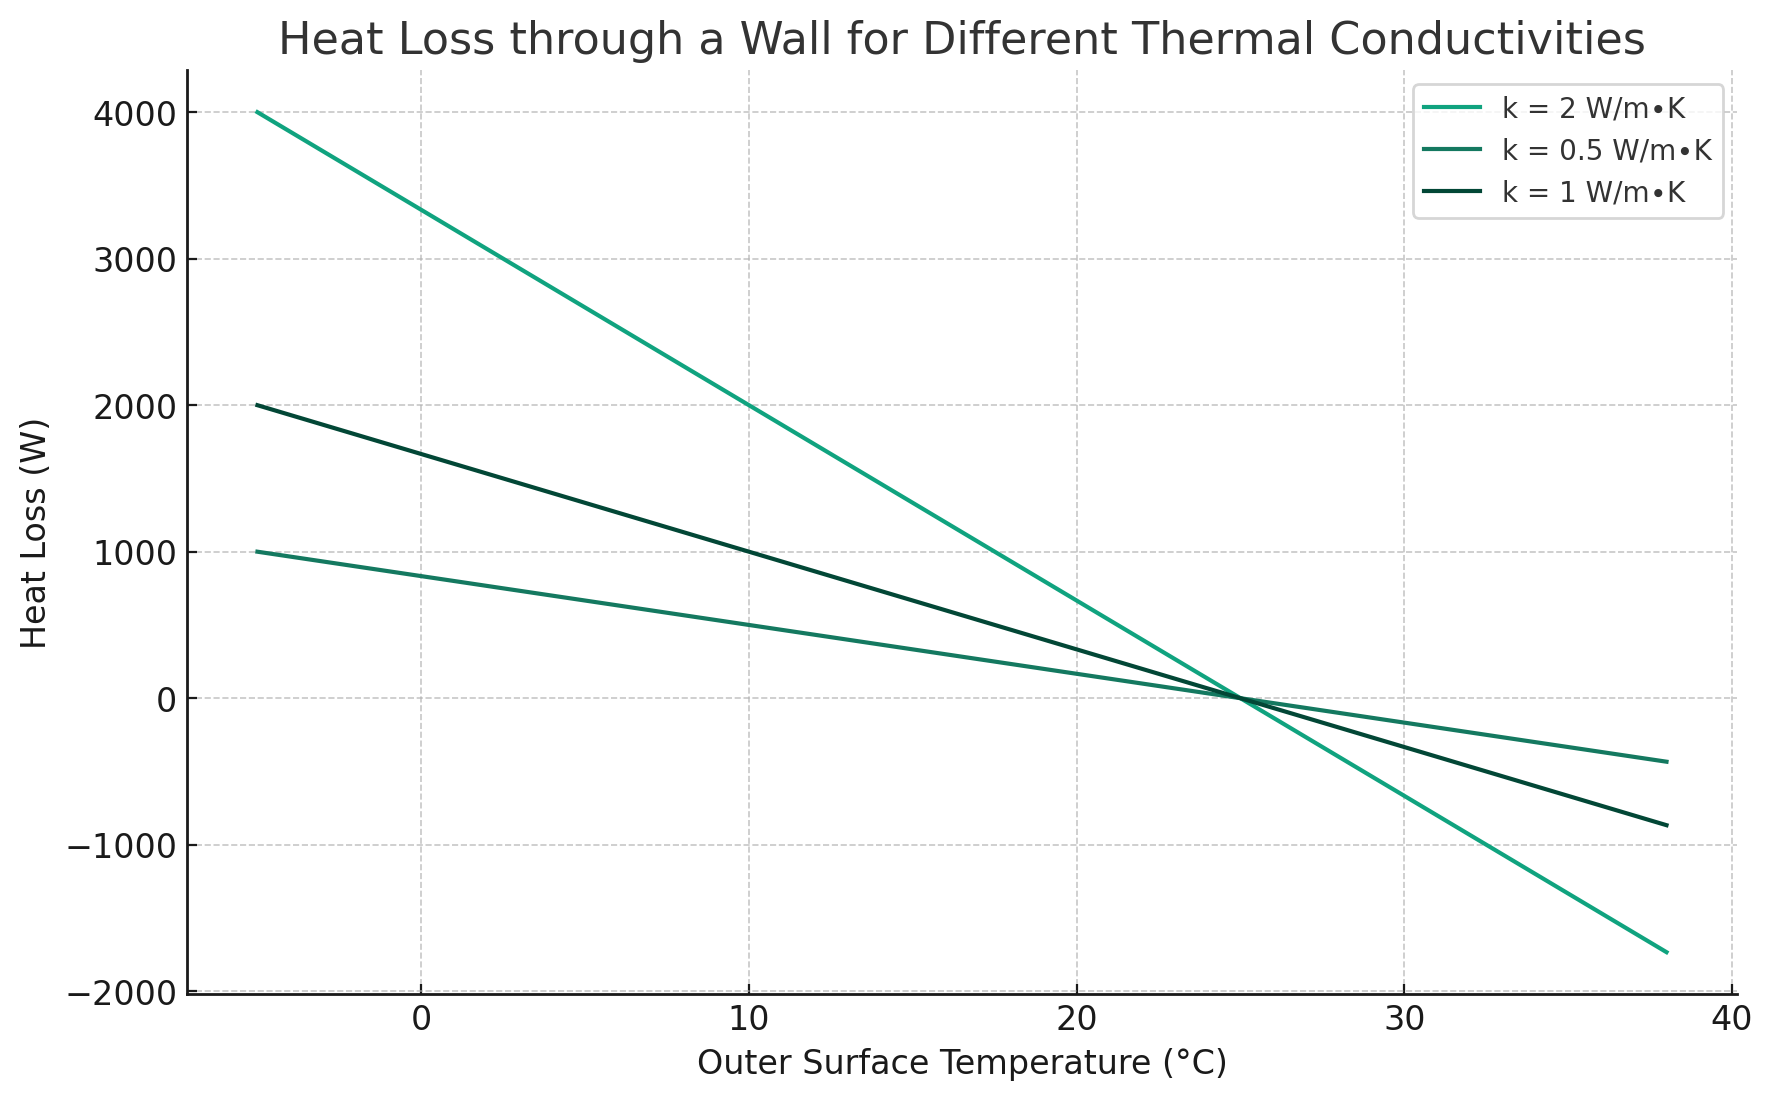
\includegraphics[width=0.9\textwidth]{354_hw1.png}
    \caption{Heat loss through a wall for different thermal conductivities}
    \label{fig:heat_loss}
\end{figure}

The graph illustrates a linear relationship between heat loss and the temperature difference across the wall. It is observed that materials with higher thermal conductivity exhibit greater heat loss, indicating their lower effectiveness as insulators. This information is crucial for optimizing thermal insulation in building design.
\newpage\section{Problem Statement}
Given the temperature profile in a solid flat plate as \( T(x) = -190x^3 + 40x^2 + 100 \) °C, with the thermal conductivity of the plate being 5 W/m∙K, the objectives are to:
\begin{itemize}
    \item Determine the temperature at \( x = 2 \) cm.
    \item Determine the heat flux, \( q'' \), at \( x = 2 \) cm.
    \item Determine the location of the maximum/minimum heat flux.
\end{itemize}

\subsection{Temperature at \( x = 2 \) cm}
To find the temperature at \( x = 2 \) cm, we first convert the distance from centimeters to meters, as the temperature profile is given in meters. Thus, \( x = 2 \) cm is equivalent to \( x = 0.02 \) m. Substituting this value into the temperature profile equation, we get:
\[ T(0.02 \, \text{m}) = -190 \times (0.02)^3 + 40 \times (0.02)^2 + 100 \]
\[ \approx 100.014 \, \text{°C} \]

\subsection{Heat Flux at \( x = 2 \) cm}
To calculate the heat flux \( q'' \) using Fourier's law, we first need to find the derivative of the temperature profile \( T(x) \) with respect to \( x \). The temperature profile is given by:
\[ T(x) = -190x^3 + 40x^2 + 100 \]

The derivative of \( T(x) \) with respect to \( x \) is:
\[ \frac{dT}{dx} = \frac{d}{dx}(-190x^3 + 40x^2 + 100) \]
\[ = -570x^2 + 80x \]

Fourier's law of heat conduction states that the heat flux \( q'' \) is proportional to the negative of the temperature gradient, given by:
\[ q'' = -k \frac{dT}{dx} \]
where \( k \) is the thermal conductivity. For \( k = 5 \) W/m∙K, the heat flux at \( x = 2 \) cm (or 0.02 m) is:
\[ q'' = -5 \times (-570 \times (0.02)^2 + 80 \times 0.02) \]
\[ \approx -6.86 \, \text{W/m}^2 \]

\subsection{Location of Maximum/Minimum Heat Flux}
The maximum or minimum heat flux occurs where the rate of change of the temperature gradient is at an extremum. This can be found by calculating the second derivative of the temperature profile \( T(x) \) and setting it to zero.

First, the temperature profile is given by:
\[ T(x) = -190x^3 + 40x^2 + 100 \]

We have already calculated the first derivative \( \frac{dT}{dx} \):
\[ \frac{dT}{dx} = -570x^2 + 80x \]

Now, we find the second derivative \( \frac{d^2T}{dx^2} \):
\[ \frac{d^2T}{dx^2} = \frac{d}{dx}(-570x^2 + 80x) \]
\[ = -1140x + 80 \]

To find the location of maximum or minimum heat flux, set \( \frac{d^2T}{dx^2} = 0 \) and solve for \( x \):
\[ -1140x + 80 = 0 \]
\[ x = \frac{80}{1140} \]
\[ \approx 0.0702 \, \text{m} \]

Converting this to centimeters, we get:
\[ x \approx 7.02 \, \text{cm} \]

This is the location of the maximum or minimum heat flux in the solid flat plate.


\subsection{Temperature Profile / Heat Flux}
\begin{figure}[h]
    \centering
    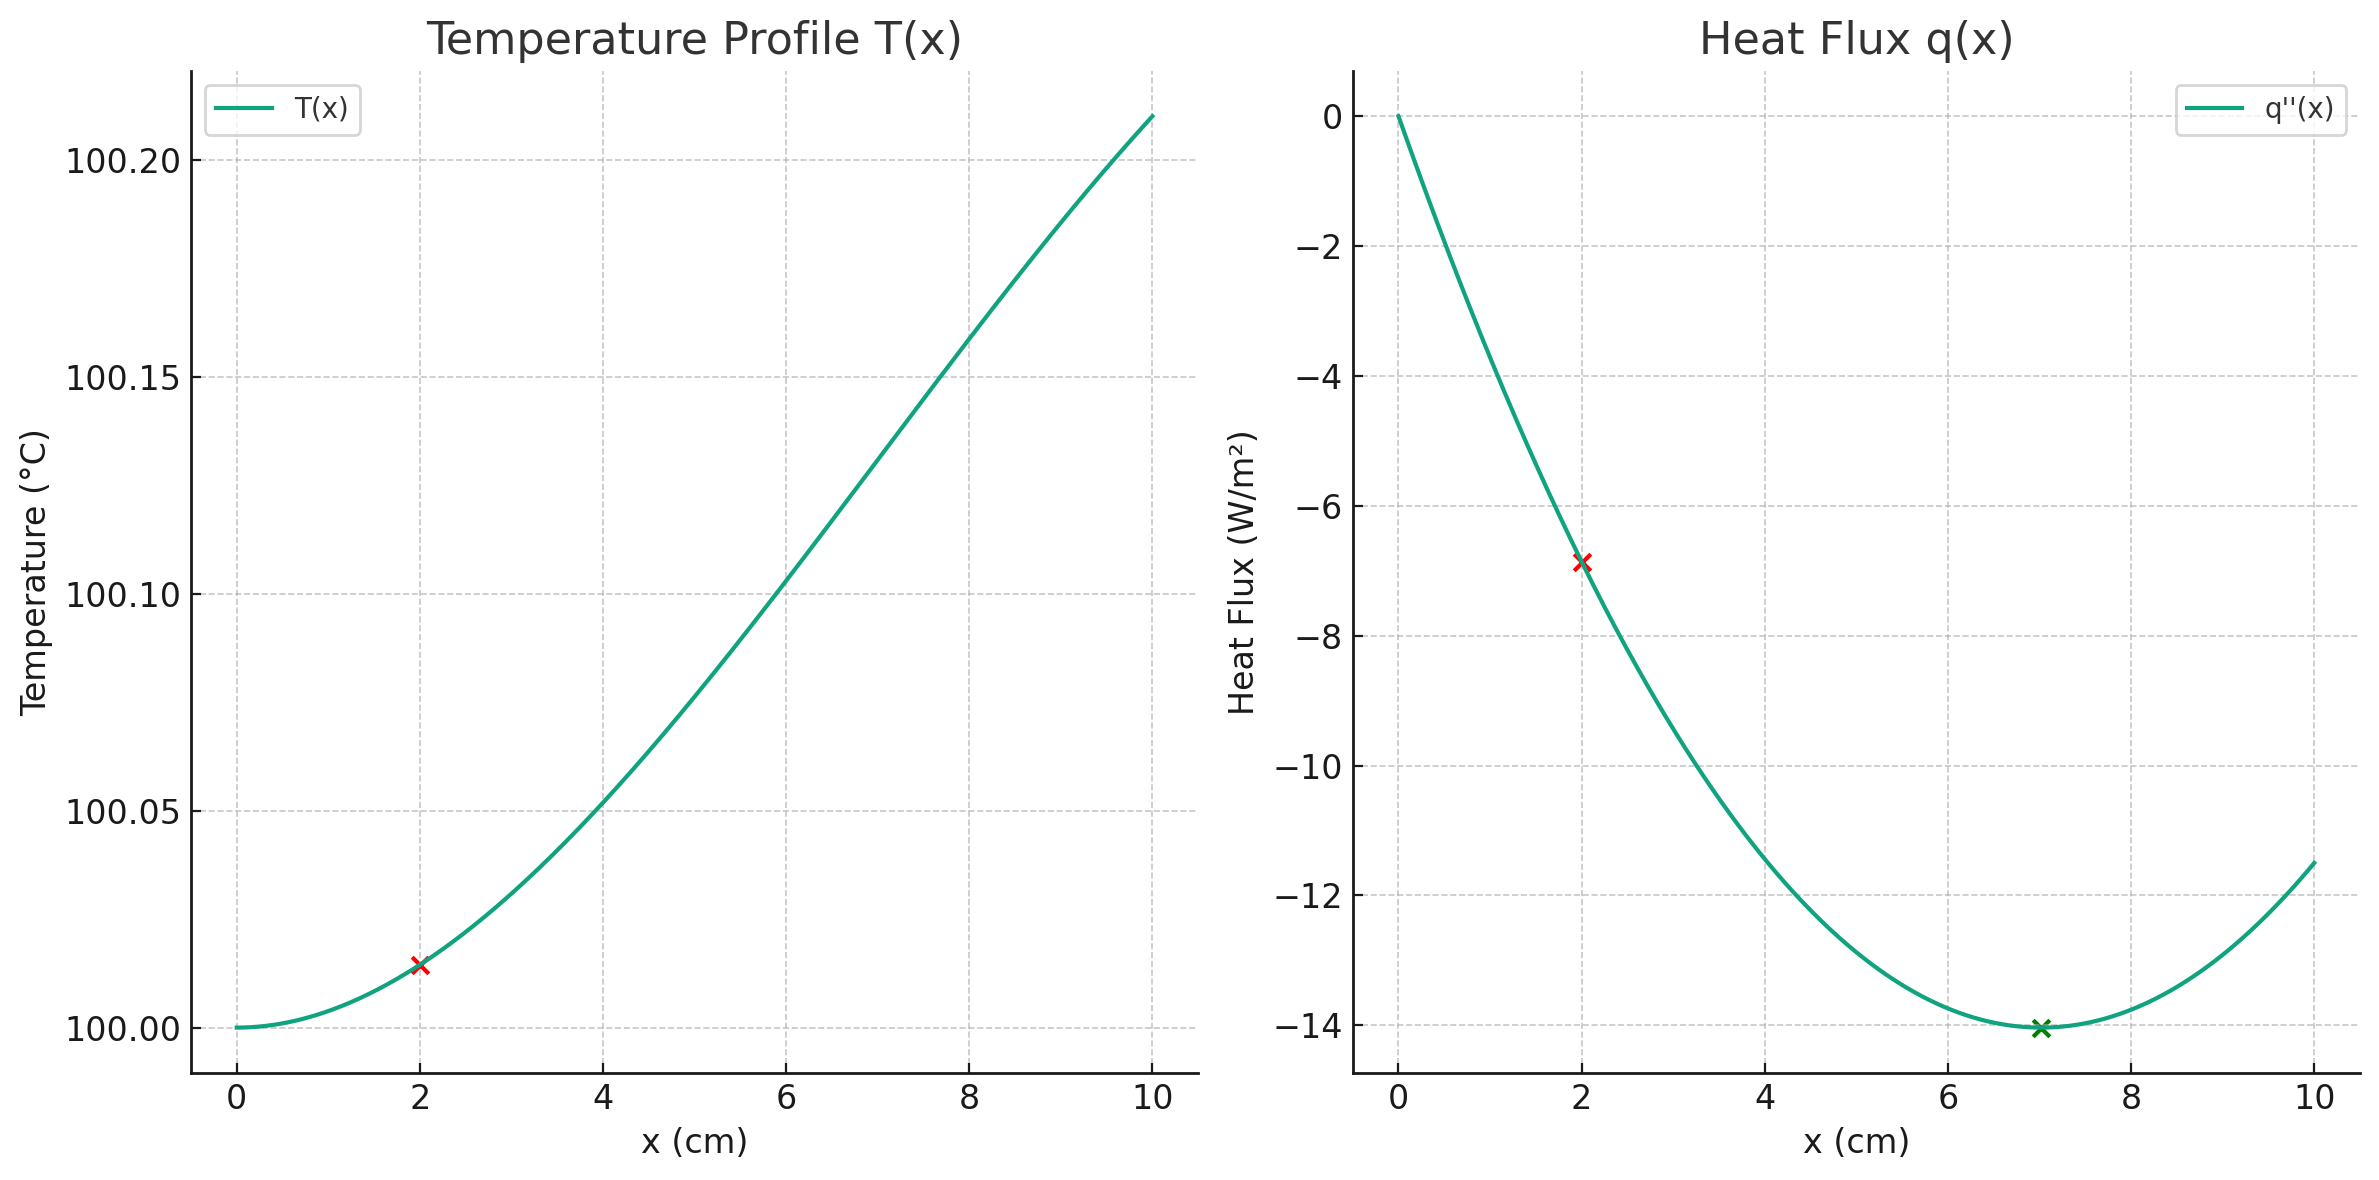
\includegraphics[width=\textwidth]{heatflux.png}
    \label{fig:temp_profile}
\end{figure}

\newpage
\section{Problem Statement}
In the boiling process depicted in Figure 1, the ambient temperature in Newton's law of cooling is replaced by the saturation temperature of the fluid. We are given a heat flux from the hot plate, \( q'' = 20 \times 10^5 \) W/m\(^2\), with water at atmospheric pressure as the fluid, and a convection heat transfer coefficient, \( h_w = 50 \times 10^3 \) W/m\(^2\cdot \) K. Our task is to determine the upper surface temperature of the plate, \( T_{s,w} \). Additionally, we explore a technician's proposal to replace water with a dielectric fluid with a saturation temperature of \( T_{sat,d} = 52 \) °C and a heat transfer coefficient \( h_d = 5 \times 10^3 \) W/m\(^2\cdot \) K to minimize the surface temperature.

\subsection{Upper Surface Temperature with Water}
Using Newton's law of cooling for boiling, modified for the saturation temperature, we have:
\[ q'' = h_w (T_{s,w} - T_{sat,w}) \]
where \( T_{sat,w} \) is the saturation temperature of water at atmospheric pressure, which is 100°C.

Rearranging to solve for \( T_{s,w} \):
\[ T_{s,w} = \frac{q''}{h_w} + T_{sat,w} \]

Substituting the given values:
\[ T_{s,w} = \frac{20 \times 10^5}{50 \times 10^3} + 100 \]
\[ T_{s,w} = 140 \, \text{°C} \]

\subsection{Upper Surface Temperature with Dielectric Fluid}
For the dielectric fluid, we similarly apply Newton's law of cooling:
\[ q'' = h_d (T_{s,d} - T_{sat,d}) \]
where \( T_{sat,d} \) is the given saturation temperature of the dielectric fluid.

Rearranging to solve for \( T_{s,d} \):
\[ T_{s,d} = \frac{q''}{h_d} + T_{sat,d} \]

Substituting the given values:
\[ T_{s,d} = \frac{20 \times 10^5}{5 \times 10^3} + 52 \]
\[ T_{s,d} = 452 \, \text{°C} \]

Since \( T_{s,d} \) is higher than \( T_{s,w} \), the technician’s proposal will not result in a lower surface temperature.
\newpage
\section{Problem Statement}
A furnace wall of thickness 0.244 m and thermal conductivity1.30 W/(m  \(\cdot\) K) is to be insulated with a material of thermal conductivity 0.356 W/(m \(\cdot\) K). The insulation must be designed such that the heat loss does not exceed 1830 W/m\(^2\). With the inner surface temperature of the wall at 1588 K and the outer surface temperature at 299 K, we must calculate the minimum thickness of the insulation required to achieve this heat loss rate.

\subsection{Thermal Resistance of the Furnace Wall}
The thermal resistance of the furnace wall, \( R_{\text{wall}} \), is given by:
\[ R_{\text{wall}} = \frac{d_{\text{wall}}}{k_{\text{wall}}} \]

Substituting in the given values:
\[ R_{\text{wall}} = \frac{0.244 \, \text{m}}{1.30 \, \text{W/(m \(\cdot\) K)}} \]
\[ R_{\text{wall}} \approx 0.1877 \, \text{m}^2\text{K/W} \]

\subsection{Maximum Allowable Thermal Resistance}
The maximum allowable thermal resistance for the entire system to maintain the heat loss rate is determined from the maximum heat flux \( q''_{\text{max}} \):
\[ R_{\text{total max}} = \frac{T_{\text{inner}} - T_{\text{outer}}}{q''_{\text{max}}} \]

\[ R_{\text{total max}} = \frac{1588 \, \text{K} - 299 \, \text{K}}{1830 \, \text{W/m}^2} \]
\[ R_{\text{total max}} \approx 0.705 \, \text{m}^2\text{K/W} \]

\subsection{Required Thickness of Insulation}
The required thickness of insulation, \( d_{\text{insulation}} \), can now be found from the remaining thermal resistance after accounting for the wall's resistance:
\[ R_{\text{insulation}} = R_{\text{total max}} - R_{\text{wall}} \]

\[ d_{\text{insulation}} = R_{\text{insulation}} \cdot k_{\text{insulation}} \]
\[ d_{\text{insulation}} = (0.705 \, \text{m}^2\text{K/W} - 0.1877 \, \text{m}^2\text{K/W}) \cdot 0.356 \, \text{W/(m \(\cdot\) K)} \]
\[ d_{\text{insulation}} \approx 0.184 \, \text{m} \]
\end{document}
